%!TEX TS-program = xelatex
%!TEX encoding = UTF-8 Unicode

\documentclass[12pt]{extarticle}
% extarticle is like article but can handle 8pt, 9pt, 10pt, 11pt, 12pt, 14pt, 17pt, and 20pt text

\def \ititle {Origins of Mind}
 
\def \isubtitle {Lecture 01}
 
\def \iauthor {Stephen A. Butterfill}
\def \iemail{s.butterfill@warwick.ac.uk}
\date{}

%for strikethrough
\usepackage[normalem]{ulem}

\input{$HOME/Documents/submissions/preamble_steve_handout}

%\bibpunct{}{}{,}{s}{}{,}  %use superscript TICS style bib
%remove hanging indent for TICS style bib
%TODO doesnt work
\setlength{\bibhang}{0em}
%\setlength{\bibsep}{0.5em}


%itemize bullet should be dash
\renewcommand{\labelitemi}{$-$}

\begin{document}

\begin{multicols}{3}

\setlength\footnotesep{1em}


\bibliographystyle{newapa} %apalike

%\maketitle
%\tableofcontents



\

\begin{center}
{\Large
\textbf{\ititle}
}

\iemail %<s.butterfill@warwick.ac.uk>

\end{center}


 
 \def \ititle {Origins of Mind}
 
\def \isubtitle {Lecture 01}
 
 
 
\textbf{Question}
How do humans come to know about---and to knowingly manipulate---objects, causes, words, numbers, colours, actions and minds?
 
‘... ’tis past doubt, that Men have in their Minds several Ideas, such as are those expressed by the words, Whiteness, Hardness, ... and others: It is in the first place to be enquired, How he comes by them?’
\citep[p.\ 104]{Locke:1975qo}
 
‘How does it come about that the development of organic behavior into controlled inquiry brings about the differentiation and cooperation of observational and conceptual operations?’
\citep[p.\ 12]{Dewey:1938yp}
 
‘the fundamental explicandum, is the organism and its propositional attitudes ... Cognitive psychologists accept ... the ... necessity of explaining how organisms come to have the attitudes to propositions that they do.’
\citep[p.\ 198]{Fodor:1975pb}
 
 
 
\section{From Myths to Mechanisms}
 
‘Men, barely by the Use of their natural Faculties, may attain to all the Knowledge they have, without the help of any innate Impressions; [...]
‘For I imagine any one will easily grant, That it would be impertinent to suppose, the Ideas of Colours innate in a Creature, to whom God hath given Sight, and a Power to receive them by the Eyes from external Objects’
\citep[p.\ 48]{Locke:1975qo}
 
 
 
\section{Inbetween mindless behaviour and thought}
 
‘We have many vocabularies for describing nature when we regard it as mindless, and we have a mentalistic vocabulary for describing thought and intentional action; what we lack is a way of describing what is in between’ \citep[p.\ 11]{Davidson:1999ju}
 
‘there are many separable systems of mental representations ... and thus many different kinds of knowledge. ... the task ... is to contribute to the enterprise of finding the distinct systems of mental representation and to understand their development and integration’
\citep[p.\ 1522]{Hood:2000bf}.
 
 
 
\section{*todo*}
 
 
 
\section{Two Breakthroughs}
 
 
 
\section{Social Interaction}
 
‘children learn words through the exercise of reason’
(\citealp[p.\ 1103]{Bloom:2001ka}; see \citealp{Bloom:2000qz})
 
‘Augustine describes the learning of human language as if the child came into a strange country and did not understand the language of the country; that is, as if it already had a language, only not this one. Or again: as if the child could already think, only not yet speak.’
\citep[15--16, §32]{Wittgenstein:1953mm}
 
‘[t]he child learns this language from the grown-ups by being trained to its use. I am using the word ‘trained’ in a way strictly analogous to that in which we talk of an animal being trained to do certain things. It is done by means of example, reward, punishment, and suchlike’
\citep[p.\ 77]{Wittgenstein:1972lj}
 
‘the child's early learning of a verbal response depends on society's reinforcement of the response in association with the stimulations that merit the response’
(\citeyear[p.\ 82]{Quine:1960fe}; compare \citeyear[pp.\ 28--9]{Quine:1974rd})
 
‘A child learning to speak is learning habits and associations which are just as much determined by the environment as the habit of expecting dogs to bark and cocks to crow’
\citep[p.\ 71]{Russell:1921ww}
 
 
 
\section{Representation}
 
\begin{center}
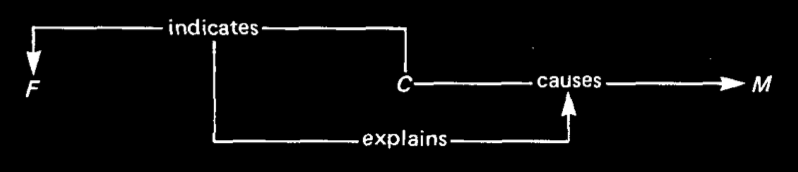
\includegraphics[scale=0.3]{../slides/src/files/img/dretske_1988_fig4.1.png}
\end{center}
source: \citep[p.\ 84, figure 4.1]{Dretske:1988sq}
 
‘Once C is recruited as a cause of M---and recruited as a cause of M because of what it indicates about F---C acquires, thereby, the function of indicating F. Hence, C comes to represent F. C acquires its semantics, a genuine meaning, at the very moment when a component of its natural meaning (the fact that it indicates F) acquires an explanatory relevance.’
\citep[p.\ 84]{Dretske:1988sq}
 
 
 
\footnotesize 
\bibliography{$HOME/endnote/phd_biblio}

\end{multicols}

\end{document}